\chapter{Memory Handlers}
\label{chap_memory}

Memory Handlers berfungsi menangani pembacaan dan penulisan data ke media penyimpanan secara umum. Pembacaan dan penulisan secara aktual dilakukan dengan memanggil fungsi HAL Memory yang sesuai. Memory menyediakan sebuah alamat virtual untuk menyimpan dan memperoleh data tanpa harus mengetahui lokasi data sebenarnya pada sistem. Konfigurasi virtual address yang digunakan tergantung pada platform smartcard yang digunakan. Gambar \ref{fig-mem-virtualaddress} menampilkan contoh konfigurasi virtual memory pada platform funcard.

\begin{table}[h]
  \centering
  \begin{tabular}{ c c c }
    \cline{3-3}
    0x001001fe &       & \multicolumn{1}{|c|}{0xfffff} \\
    \cline{3-3}
               &       & \multicolumn{1}{|c|}{}        \\
               &       & \multicolumn{1}{|c|}{}        \\
               &       & \multicolumn{1}{|c|}{.....}   \\
               &       & \multicolumn{1}{|c|}{}        \\
               &       & \multicolumn{1}{|c|}{}        \\
    \cline{3-3}
    0x00000200 &       & \multicolumn{1}{|c|}{0x00000} \\
    \cline{2-2}\cline{3-3}
    0x000001ff & \multicolumn{1}{|c|}{0x1ff} &         \\
    \cline{2-2}
               & \multicolumn{1}{|c|}{}      &         \\
               & \multicolumn{1}{|c|}{.....} &         \\
               & \multicolumn{1}{|c|}{}      &         \\
    \cline{2-2}
    0x00000000 & \multicolumn{1}{|c|}{0x000} &         \\
    \cline{2-2}
    \bf{Virtual Address} & \bf{Internal Memory} & \bf{External Memory} \\
  \end{tabular}
  \caption{Contoh konfigurasi virtual address pada platform funcard}
  \label{tabel-func-memory}
\end{table}

Pada file konfigurasi, ukuran (batas atas) virtual memory dinyatakan sebagai MEMORY\_SIZE, dan batas antara bagian virtual memory yang menggunakan Internal dan Eksternal Memory dinyatakan sebagai INTERNAL\_MEMORY\_SIZE.

Memory Handlers menyediakan sejumlah interface yang dapat digunakan bagian pintarOS lainnya (terutama File System) sebagai metode pembacaan/penulisan sebagaimana didaftarkan pada Tabel \ref{fig-func-memory}.

\begin{table}[h]
  \centering
  \begin{tabular}{|m{5cm}|m{8cm}|}
    \hline
    \bf{Nama Fungsi} & \bf{Kegunaan} \\
    \hline
    Read Byte & Membaca 1 byte data dari alamat virtual \\
    \hline
    Write Byte & Menulis 1 byte data ke alamat virtual \\
    \hline
    Read Block & Membaca 1 block data dari alamat virtual \\
    \hline
    Write Block & Menulis 1 block data ke alamat virtual \\
    \hline
  \end{tabular}
  \caption{Daftar antarmuka fungsi yang disediakan Memory Handlers}
  \label{tabel-func-memory}
\end{table}

\section{Memory Read Byte}
\label{sec_memoryreadbyte}

Berfungsi membaca 1 byte data dari Memory EEPROM (internal & eksternal). Gambar \ref{fig-dfd-readbyte} menampilkan DFD dari fungsi Memory Read Byte (ReadByte). Diagram alir fungsi kemudian ditampilkan pada Gambar \ref{fig-flow-readbyte}. Fungsi ini pertama akan mencari lokasi memory yang akan dibaca dari alamat yang diberikan, apakah terdapat pada memory internal atau eksternal. Setelah mengetahui lokasi memory yang akan dibaca, fungsi ini akan memanggil fungsi HAL yang sesuai yang kemudian akan membaca byte data secara aktual dari lokasi memory.

\begin{figure}[!h]
\centering
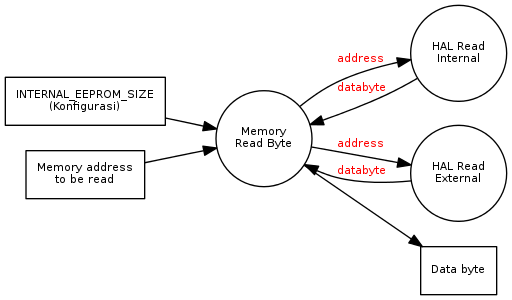
\includegraphics[width=0.75\textwidth]{image/memory/dfd_readbyte.png}
\caption{DFD Memory Read Byte}
\label{fig-dfd-readbyte}
\end{figure}

\begin{figure}[!h]
\centering
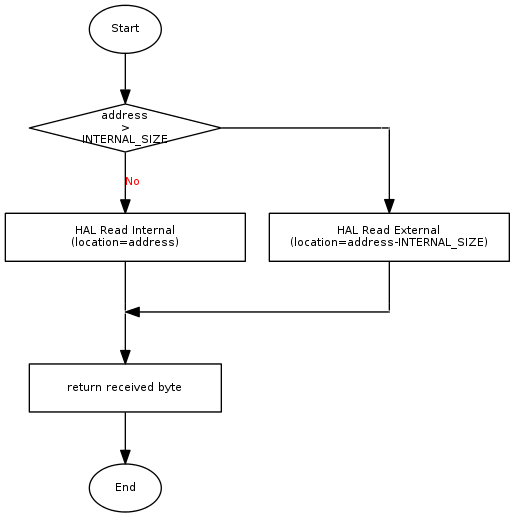
\includegraphics[width=0.75\textwidth]{image/memory/flow_readbyte.png}
\caption{Flowchart Memory Read Byte}
\label{fig-flow-readbyte}
\end{figure}

\subsection {Pengujian}

\begin{table}[!h]
  \centering
  \begin{tabular}{ | c || c | }
    \hline
    \bf{Input}  & \bf{Output} \\
    \hline
    \bf{address} & \bf{Return Value}\\
    \hline
    \multicolumn{2}{ |c| }{Filled internal and external memory according to their virtual address} \\
    \multicolumn{2}{ |c| }{} \\
    \multicolumn{2}{ |c| }{
      \begin{tabular}{ c | c | }
        \cline{2-2}
        0x0000 - 0x000f & 0x00, 0x01, ..., 0x0f \\
        \cline{2-2}
        0x0010 - 0x001f & 0x10, 0x11, ..., 0x1f \\
        \cline{2-2}
        & ... \\
        \cline{2-2}
        0x00f0 - 0x00ff & 0xf0, 0xf1, ..., 0xff \\
        \cline{2-2}
        0x0100 - 0x010f & 0x00, 0x01, ..., 0x0f \\
        \cline{2-2}
        0x0110 - 0x011f & 0x10, 0x11, ..., 0x1f \\
        \cline{2-2}
        & ... \\
        \cline{2-2}
        0xfff0 - 0xffff & 0xf0, 0xf1, ..., 0xff \\
        \cline{2-2}
      \end{tabular}
    } \\
    \multicolumn{2}{ |c| }{} \\

    \hline
    0x0000 & = 0x00 \\
    0x0001 & = 0x01 \\
    \hline
    \multicolumn{2}{ |c| }{...} \\
    \hline
    0x00ff & = 0xff \\
    0x0100 & = 0x00 \\
    0x0101 & = 0x01 \\
    \hline
    \multicolumn{2}{ |c| }{...} \\
    \hline
    0x01ff & = 0xff \\
    \hline
    \multicolumn{2}{ |c| }{...} \\
    \hline
    0xff00 & = 0x00 \\
    0xff01 & = 0x01 \\
    \hline
    \multicolumn{2}{ |c| }{...} \\
    \hline
    0xffff & = 0xff \\
    \hline
    \multicolumn{2}{ |c| }{...} \\
    \hline
    0xff & = 0xff \\
    \hline
  \end{tabular}
  \caption{Test Vector Fungsi Memory Read Byte}
  \label{tabel-test-readbyte}
\end{table}

Tabel \ref{tabel-test-readbyte} menampilkan Test Vector yang digunakan untuk menguji fungsi Memory Read Byte.

\subsection {Implementasi}

Tabel \ref{tabel-readbyte} menampilkan purwarupa dari implementasi fungsi Memory Read Byte

\begin{table}[h]
  \centering
  \begin{tabular}{p{2cm} p{8cm}}
    \hline\\
    {\bf Name} & Memory\_ReadByte\\
    \hline\\
    {\bf Input} & alamat memory virtual yang akan dibaca
    \\
    \hline\\
    {\bf Output} & data hasil pembacaan (1 byte)
    \\
    \hline
  \end{tabular}
  \caption{Prototype Fungsi Memory Read Byte}
  \label{tabel-readbyte}
\end{table}

Listing \ref{list-readbyte} menampilkan potongan program yang mengimplementasi fungsi Memory Read Byte.

\begin{lstlisting}[caption={Listing Program Fungsi Memory Read Byte}, label={list-readbyte}]
uint8_t Memory_ReadByte(uint16_t address)
{
  if( address < INTERNAL_EEPROM_SIZE )
    {
      return readinternalmem(address);
    }
  else
    {
      return readexternalmem(address - INTERNAL_EEPROM_SIZE);
    }
}
\end{lstlisting}

\section{Memory Write Byte}
\label{sec_memorywritebyte}

Berfungsi menulis 1 byte data ke Memory EEPROM (internal & eksternal). Gambar \ref{fig-dfd-writebyte} menampilkan DFD dari fungsi Memory Write Byte (WriteByte). Diagram alir fungsi kemudian ditampilkan pada Gambar \ref{fig-flow-writebyte}. Fungsi ini pertama akan mencari lokasi memory yang akan ditulis dari alamat yang diberikan, apakah terdapat pada memory internal atau eksternal. Setelah mengetahui lokasi memory yang akan ditulis, fungsi ini akan memanggil sebuah fungsi HAL yang sesuai yang akan secara aktual menulis byte data ke lokasi memory.

\begin{figure}[!h]
\centering
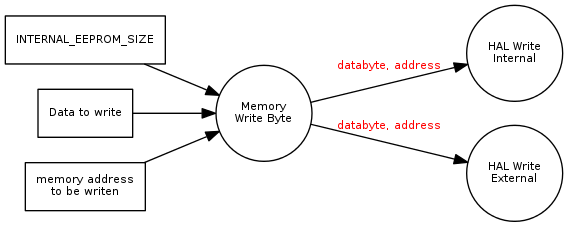
\includegraphics[width=0.75\textwidth]{image/memory/dfd_writebyte.png}
\caption{DFD Memory Write Byte}
\label{fig-dfd-writebyte}
\end{figure}

\begin{figure}[!h]
\centering
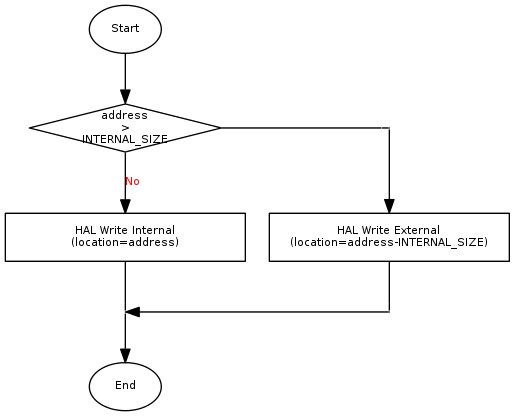
\includegraphics[width=0.75\textwidth]{image/memory/flow_writebyte.png}
\caption{Flowchart Memory Write Byte}
\label{fig-flow-writebyte}
\end{figure}

\subsection {Pengujian}

\begin{table}[!h]
  \centering
  \begin{tabular}{ | c | c || c | }
    \hline
    \multicolumn{2}{ |c|| }{\bf{Input}}  & \bf{Output} \\
    \hline
    \bf{address} & \bf{data} & \bf{Memory value @address}\\
    0x0000 & 0x00 & = 0x00 \\
    \hline
    \multicolumn{3}{ |c|| }{...}\\
    \hline
    0x000f & 0x0f & = 0x0f \\
    0x0010 & 0x10 & = 0x10 \\
    \hline
    \multicolumn{3}{ |c|| }{...}\\
    \hline
    0x001f & 0x1f & = 0x1f \\
    \hline
    \multicolumn{3}{ |c|| }{...}\\
    \hline
    0x00ff & 0xff & = 0xff \\
    0x0100 & 0x00 & = 0x00 \\
    \hline
    \multicolumn{3}{ |c|| }{...}\\
    \hline
    0x01ff & 0xff & = 0xff \\
    \hline
    \multicolumn{3}{ |c|| }{...}\\
    \hline
    0x0fff & 0xff & = 0xff \\
    0x1f00 & 0x00 & = 0x00 \\
    \hline
    \multicolumn{3}{ |c|| }{...}\\
    \hline
    0x1fff & 0xff & = 0xff \\
    \hline
    \multicolumn{3}{ |c|| }{...}\\
    \hline
    0xffff & 0xff & = 0xff \\
    \hline
  \end{tabular}
  \caption{Test Vector Fungsi Memory Write Byte}
  \label{tabel-test-writebyte}
\end{table}

Tabel \ref{tabel-test-writebyte} menampilkan Test Vector yang digunakan untuk menguji fungsi Memory Write Byte.

\subsection {Implementasi}

Tabel \ref{tabel-writebyte} menampilkan purwarupa dari implementasi fungsi Memory Write Byte 

\begin{table}[!h]
  \centering
  \begin{tabular}{p{2cm} p{8cm}}
    \hline\\
    {\bf Name} & Memory\_WriteByte\\
    \hline\\
    {\bf Input} & 
    \begin{itemize}[noitemsep,topsep=0pt,parsep=0pt,partopsep=0pt]
    \item alamat memory yang akan ditulis
    \item data yang akan ditulis (1 byte)
    \end{itemize}
    \\
    \hline\\
    {\bf Output} & -
    \\
    \hline
  \end{tabular}
  \caption{Prototype Fungsi Memory Write Byte}
  \label{tabel-writebyte}
\end{table}

Listing \ref{list-writebyte} menampilkan potongan program yang mengimplementasi fungsi Memory Write Byte.

\begin{lstlisting}[caption={Listing Program Fungsi Memory Write Byte}, label={list-writebyte}]
void Memory_WriteByte(uint16_t address, uint8_t databyte)
{
  if( address < INTERNAL_EEPROM_SIZE )
    {
      writeinternalmem(address, databyte);
    }
  else
    {
      writeexternalmem(address - INTERNAL_EEPROM_SIZE, databyte);
    }
}
\end{lstlisting}

\section{Memory Read Block}
\label{sec_memoryreadblock}

Berfungsi membaca 1 block data dari Memory EEPROM (internal & eksternal). Gambar \ref{fig-dfd-readblock} menampilkan DFD dari fungsi Memory Read Block (ReadBlock). Diagram alir fungsi kemudian ditampilkan pada Gambar \ref{fig-flow-readblock}. Fungsi ini akan membaca memory dimulai dari alamat memory yang diberikan berturut-turut sepanjang \emph{len} byte dengan memanggil fungsi Read Byte.

\begin{figure}[!h]
\centering
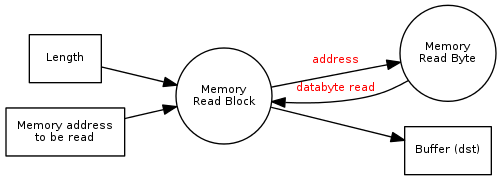
\includegraphics[width=0.75\textwidth]{image/memory/dfd_readblock.png}
\caption{DFD Memory Read Block}
\label{fig-dfd-readblock}
\end{figure}

\begin{figure}[!h]
\centering
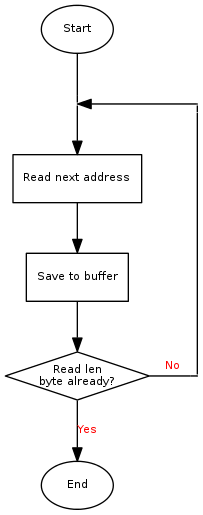
\includegraphics[height=0.5\textheight]{image/memory/flow_readblock.png}
\caption{Flowchart Memory Read Block}
\label{fig-flow-readblock}
\end{figure}

\subsection {Pengujian}

\begin{table}[!h]
  \centering
  \begin{tabular}{ | c | c || c | }
    \hline
    \multicolumn{2}{| c ||}{\bf{Input}}  & \bf{Output} \\
    \hline
    \bf{address} & \bf{length} & \bf{Output buffer}\\
    \hline
    \multicolumn{3}{ |c| }{Filled internal and external memory according to their virtual address} \\
    \multicolumn{3}{ |c| }{} \\
    \multicolumn{3}{ |c| }{
      \begin{tabular}{ c | c | }
        \cline{2-2}
        0x0000 - 0x000f & 0x00, 0x01, ..., 0x0f \\
        \cline{2-2}
        0x0010 - 0x001f & 0x10, 0x11, ..., 0x1f \\
        \cline{2-2}
        & ... \\
        \cline{2-2}
        0x00f0 - 0x00ff & 0xf0, 0xf1, ..., 0xff \\
        \cline{2-2}
        0x0100 - 0x010f & 0x00, 0x01, ..., 0x0f \\
        \cline{2-2}
        0x0110 - 0x011f & 0x10, 0x11, ..., 0x1f \\
        \cline{2-2}
        & ... \\
        \cline{2-2}
        0xfff0 - 0xffff & 0xf0, 0xf1, ..., 0xff \\
        \cline{2-2}
      \end{tabular}
    } \\
    \multicolumn{3}{ |c| }{} \\
    \hline
    0x0000 & 0x0001 & = [0x00] \\
    0x0001 & 0x000e & = [0x01, 0x02, ..., 0x0f] \\
    0x0010 & 0x00ef & = [0x10, 0x11, ..., 0xff] \\
    0x0100 & 0x0eff & = [0x00, 0x01, ..., 0xff]x15 \\
    0x1000 & 0xefff & = [0x00, 0x01, ..., 0xff]x239 \\
    \hline
  \end{tabular}
  \caption{Test Vector Fungsi Memory Read Block}
  \label{tabel-test-readblock}
\end{table}

Tabel \ref{tabel-test-readblock} menampilkan Test Vector yang digunakan untuk menguji fungsi Memory Read Block.

\subsection {Implementasi}

\begin{table}[!h]
  \centering
  \begin{tabular}{p{2cm} p{8cm}}
    \hline\\
    {\bf Name} & Memory\_ReadBlock\\
    \hline\\
    {\bf Input} & 
    \begin{itemize}[noitemsep,topsep=0pt,parsep=0pt,partopsep=0pt]
    \item awal alamat virtual memory yang akan dibaca
    \item panjang data yang akan dibaca
    \item alamat buffer dimana data akan disimpan
    \end{itemize}
    \\
    \hline\\
    {\bf Output} & jumlah byte yang terbaca
    \\
    \hline
  \end{tabular}
  \caption{Prototype Fungsi Memory Read Block}
  \label{tabel-readblock}
\end{table}

Tabel \ref{tabel-readblock} menampilkan purwarupa dari implementasi fungsi Memory ReadBlock. Listing \ref{list-readblock} menampilkan potongan program yang mengimplementasi fungsi Memory Read Block.

\begin{lstlisting}[caption={Listing Program Fungsi Memory Read Block}, label={list-readblock}]
int Memory_ReadBlock(uint16_t address, uint16_t size, uint8_t * databyte)
{
  uint16_t count;

  for( count=0; count < size; count++)
    {
      *(databyte+count) = Memory_ReadByte(address+count);
    }

  return count;
}
\end{lstlisting}

\section{Memory Write Block}
\label{sec_memorywriteblock}

Berfungsi menulis 1 block data ke Memory EEPROM (internal & eksternal). Gambar \ref{fig-dfd-writeblock} menampilkan DFD dari fungsi Memory Write Block (WriteBlock). Diagram alir fungsi kemudian ditampilkan pada Gambar \ref{fig-flow-writeblock}. Fungsi ini akan menulis data dari buffer ke memory dimulai dari alamat memory yang diberikan berturut-turut sepanjang \emph{len} byte dengan memanggil fungsi Memory Write Byte.

\begin{figure}[!h]
\centering
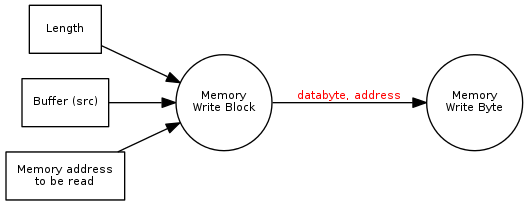
\includegraphics[width=0.75\textwidth]{image/memory/dfd_writeblock.png}
\caption{DFD Memory Write Block}
\label{fig-dfd-writeblock}
\end{figure}

\begin{figure}[!h]
\centering
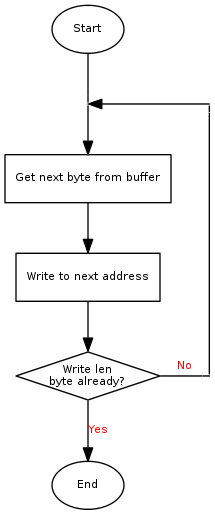
\includegraphics[height=0.5\textheight]{image/memory/flow_writeblock.png}
\caption{Flowchart Memory Write Block}
\label{fig-flow-writeblock}
\end{figure}

\subsection {Pengujian}

\begin{table}[!h]
  \centering
  \begin{tabular}{ | c | c | c || c | }
    \hline
    \multicolumn{3}{ |c|| }{\bf{Input}}  & \bf{Output} \\
    \hline
    \bf{address} & \bf{data} & \bf{length} & \bf{Memory value @address$\to$address+length}\\
    \hline
    0x0000 & [0x00] & 0x0001 & = [0x00] \\
    0x0001 & [0x01, ..., 0x0f] & 0x000e & = [0x01, ..., 0x0f] \\
    0x0010 & [0x10, ..., 0xff] & 0x00ef & = [0x10, ..., 0xff] \\
    0x0100 & [0x00, ..., 0xff]X15 & 0x0eff & = [0x00, ..., 0xff]X15 \\
    0x1000 & [0x00, ..., 0xff]X239 & 0xefff & = [0x00, ..., 0xff]X239 \\
    \hline
  \end{tabular}
  \caption{Test Vector Fungsi Memory Write Block}
  \label{tabel-test-writeblock}
\end{table}

Tabel \ref{tabel-test-writeblock} menampilkan Test Vector yang digunakan untuk menguji fungsi Memory Write Block.


\subsection {Implementasi}

\begin{table}[!h]
  \centering
  \begin{tabular}{p{2cm} p{8cm}}
    \hline\\
    {\bf Name} & Memory Write Block\\
    \hline\\
    {\bf Input} & 
    \begin{itemize}[noitemsep,topsep=0pt,parsep=0pt,partopsep=0pt]
    \item awal alamat memory virtual yang akan ditulis
    \item alamat buffer data yang akan ditulis
    \end{itemize}
    \\
    \hline\\
    {\bf Output} & jumlah byte yang berhasil ditulis
    \\
    \hline
  \end{tabular}
  \caption{Prototype Fungsi Memory Write Block}
  \label{tabel-writeblock}
\end{table}

Tabel \ref{tabel-writeblock} menampilkan purwarupa dari implementasi fungsi Memory Write Block. Listing \ref{list-writeblock} menampilkan potongan program yang mengimplementasi fungsi Memory Write Block.

\begin{lstlisting}[caption={Listing Program Fungsi Memory Write Block}, label={list-writeblock}]
int Memory_WriteBlock(uint16_t address, uint16_t size, uint8_t * databyte)
{
  uint16_t count;

  for( count=0; count < size; count++)
    {
      Memory_WriteByte(address+count, *(databyte+count));
    }

  return count;
}
\end{lstlisting}
